\section{Introduction}\label{sec:introduction}

Smart contracts are computer programs that get executed
inside the nodes of a blockchain network. They express some form of
agreement among parties, that gets enforced by the properties of the
underlying
blockchain. Namely, the blockchain's data immutability and its consensus
algorithm make it hard
to violate the rules of the protocol, replace data
or censure specific transactions.
While this is desirable for protocols that must hold
and resist in the wild, it also means that code bugs, if present,
are also enforced and cannot be patched.
Therefore, it is highly relevant to deploy smart contracts
only if they do not contain software bugs.
There is large literature about bugs that led to
protocol breaches and stolen money (just for the case of Ethereum,
see for instance~\cite{AntonopoulosW25}).
The always cited example of reentrancy shows that attacks to
smart contracts can actually be rather involved and exploit
misunderstood features of the programming language.
In general, the use of Turing-complete programming languages
for writing smart contracts is welcome, but increases the risk
of writing buggy code and lose money. The use of
new programming languages, sometimes with vague or misleading semantics,
further complicates the programming task.

A source of bugs in smart contracts comes from the completely different
way of interaction \wrt traditional software for desktop computers. Namely,
smart contracts operate in the wild. After deployment, their API can
be called in any order and with any argument. There is no such a thing
as a \emph{correct} or \emph{expected} use of a function: users (and attackers)
may call public functions in any order and with any allowed argument.
In this sense, smart contracts are more similar to old-fashioned
servlets and to general-purpose libraries than to traditional software
for desktop computers. Their development requires a careful analysis of their
API and an extensive use of defensive programming, that should foresee all
possible illegal uses. Not surprisingly, many developers,
often unexperienced juniors who jumped on the promising business
of smart contract development,
got overwhelmed by this complexity. Bugs thrived. Money got lost.

This paper focuses on a specific, frequent bug of smart contracts.
Namely, smart contracts often store data in containers, such as lists,
that can be \emph{arbitrarily large}.
This is fine as long as such containers do not get
iterated. Otherwise, the iteration loop might have an arbitrarily large
gas cost, even larger than the maximal gas cost
allowed for a single smart contract transaction.
If that happens, the iteration always fail for gas exhaustion, which might block
some smart contract functionality and, in some case,
even lock money in the contract, forever. The goal of this paper is
to define a static program analysis that guarantees, automatically,
that there exists a maximal size for iterated containers,
for all possible ways of calling the API of a smart contract.
We call such containers \emph{bounded} and the proposed verification technique
is consequently a \emph{boundedness analysis}. Note that
a specific boundedness analysis
does not necessarily compute the exact gas cost for each API function.
If ever possible, that would be a much more concrete analysis,
in terms of abstract interpretation,
with higher cost, more difficulties
and challenges. Boundedness analysis just guarantees the existence
of a bound for the iterated containers. It is up to the programmer
to verify that that bound is small enough for the specific blockchain
at hand. In this sense, boundedness analysis remains blockchain-agnostic.

The specific boundedness analysis defined in this paper
is a sound analysis based on
an abstract interpretation of the trace semantics of the public API
of the smart contract into a set of linear constraints that express
the size change of the iterated containers. Such constraints are
subsequently fed into a theorem prover, that tries to establish
if a maximal bound
exists for the containers. The soundness guarantee is that,
if the theorem prover finds that bound, then
the code does not suffer from boundedness bugs.

The contributions of this paper are:
%
\begin{enumerate}
\item a formal definition of the boundedness property for iterated containers;
\item a sound boundedness analysis, based on abstract interpretation;
\item a prototype implementation for a minimalistic smart contract language.
\end{enumerate}

\begin{figure}[b]
  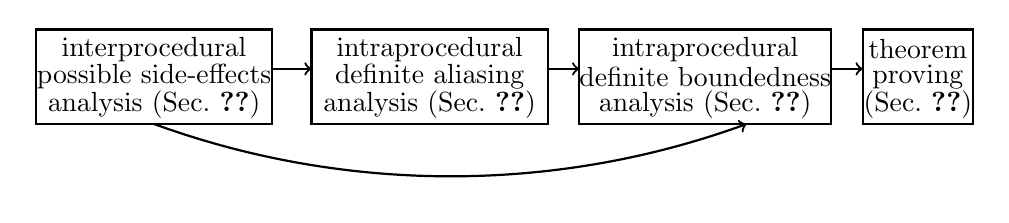
\begin{tikzpicture}
    \draw [thick] (0,0) rectangle +(3,1.2);
    \draw (1.5,0.95) node{interprocedural};
    \draw (1.5,0.6) node{possible side-effects};
    \draw (1.5,0.25) node{analysis (Sec.~\ref{sec:side_effect})};

    \draw[->,thick] (3,0.7) -- +(0.5,0);
    \draw[->,thick] (1.5,0) arc (250:290:11);

    \draw [thick] (3.5,0) rectangle +(3,1.2);
    \draw (5,0.95) node{intraprocedural};
    \draw (5,0.6) node{definite aliasing};
    \draw (5,0.25) node{analysis (Sec.~\ref{sec:aliasing})};

    \draw[->,thick] (6.5,0.7) -- +(0.4,0);

    \draw [thick] (6.9,0) rectangle +(3.2,1.2);
    \draw (8.5,0.95) node{intraprocedural};
    \draw (8.5,0.6) node{definite boundedness};
    \draw (8.5,0.25) node{analysis (Sec.~\ref{sec:boundedness})};

    \draw[->,thick] (10.1,0.7) -- +(0.4,0);

    \draw [thick] (10.5,0) rectangle +(1.4,1.2);
    \draw (11.2,0.95) node{theorem};
    \draw (11.2,0.6) node{proving};
    \draw (11.2,0.25) node{(Sec.~\ref{sec:theorem_prover})};

    %\draw [fill=VioletRed, thick] (0,3.5) rectangle (4,5.5);
  \end{tikzpicture}
  \caption{The components of our boundedness analysis and their dependencies.}
  \label{fig:plan}
\end{figure}

Fig.~\ref{fig:plan} shows the dependencies of the various components of our
boundedness analysis. A preliminary side-effect analysis identifies which lists
might be modified by the execution of the commands. This information is used in
a subsequent aliasing analysis. Both are then used for the actual boundedness analysis,
whose results are sent to a theorem prover, that uses them to prove that there is
no boundedness bug in the program.

The rest of the paper is organized as follows.
Sec.~\ref{sec:examples} presents examples of bounded and unbounded containers
in actual smart contracts, and the potential attacks in case of unboundedness.
Sec.~\ref{sec:syntax} presents the syntax of a minimalistic language for
smart contracts.
Sec.~\ref{sec:side_effect} and \ref{sec:aliasing} define the supporting
side-effect ans aliasing analysis, respectively.
Sec.~\ref{sec:boundedness} defines the actual boundedness
analysis that builds on those two supporting analyses.
Sec.~\ref{sec:theorem_prover} shows how the results of the boundedness
analysis is used to generate constraints that are fed into a theorem
prover. Sec.~\ref{sec:implementation} reports preliminary results
with our prototype implementation.
Sec.~\ref{sec:related} discusses related work. Sec.~\ref{sec:conclusion} concludes.
